\documentclass[
  stu,
  longtable,
  nolmodern,
  notxfonts,
  notimes,
  colorlinks=true,linkcolor=blue,citecolor=blue,urlcolor=blue]{apa7}

\usepackage{amsmath}
\usepackage{amssymb}



\usepackage[bidi=default]{babel}
\babelprovide[main,import]{spanish}


% get rid of language-specific shorthands (see #6817):
\let\LanguageShortHands\languageshorthands
\def\languageshorthands#1{}

\RequirePackage{longtable}
\RequirePackage{threeparttablex}

\makeatletter
\renewcommand{\paragraph}{\@startsection{paragraph}{4}{\parindent}%
	{0\baselineskip \@plus 0.2ex \@minus 0.2ex}%
	{-.5em}%
	{\normalfont\normalsize\bfseries\typesectitle}}

\renewcommand{\subparagraph}[1]{\@startsection{subparagraph}{5}{0.5em}%
	{0\baselineskip \@plus 0.2ex \@minus 0.2ex}%
	{-\z@\relax}%
	{\normalfont\normalsize\bfseries\itshape\hspace{\parindent}{#1}\textit{\addperi}}{\relax}}
\makeatother




\usepackage{longtable, booktabs, multirow, multicol, colortbl, hhline, caption, array, float, xpatch}
\setcounter{topnumber}{2}
\setcounter{bottomnumber}{2}
\setcounter{totalnumber}{4}
\renewcommand{\topfraction}{0.85}
\renewcommand{\bottomfraction}{0.85}
\renewcommand{\textfraction}{0.15}
\renewcommand{\floatpagefraction}{0.7}

\usepackage{tcolorbox}
\tcbuselibrary{listings,theorems, breakable, skins}
\usepackage{fontawesome5}

\definecolor{quarto-callout-color}{HTML}{909090}
\definecolor{quarto-callout-note-color}{HTML}{0758E5}
\definecolor{quarto-callout-important-color}{HTML}{CC1914}
\definecolor{quarto-callout-warning-color}{HTML}{EB9113}
\definecolor{quarto-callout-tip-color}{HTML}{00A047}
\definecolor{quarto-callout-caution-color}{HTML}{FC5300}
\definecolor{quarto-callout-color-frame}{HTML}{ACACAC}
\definecolor{quarto-callout-note-color-frame}{HTML}{4582EC}
\definecolor{quarto-callout-important-color-frame}{HTML}{D9534F}
\definecolor{quarto-callout-warning-color-frame}{HTML}{F0AD4E}
\definecolor{quarto-callout-tip-color-frame}{HTML}{02B875}
\definecolor{quarto-callout-caution-color-frame}{HTML}{FD7E14}

%\newlength\Oldarrayrulewidth
%\newlength\Oldtabcolsep


\usepackage{hyperref}




\providecommand{\tightlist}{%
  \setlength{\itemsep}{0pt}\setlength{\parskip}{0pt}}
\usepackage{longtable,booktabs,array}
\usepackage{calc} % for calculating minipage widths
% Correct order of tables after \paragraph or \subparagraph
\usepackage{etoolbox}
\makeatletter
\patchcmd\longtable{\par}{\if@noskipsec\mbox{}\fi\par}{}{}
\makeatother
% Allow footnotes in longtable head/foot
\IfFileExists{footnotehyper.sty}{\usepackage{footnotehyper}}{\usepackage{footnote}}
\makesavenoteenv{longtable}

\usepackage{graphicx}
\makeatletter
\def\maxwidth{\ifdim\Gin@nat@width>\linewidth\linewidth\else\Gin@nat@width\fi}
\def\maxheight{\ifdim\Gin@nat@height>\textheight\textheight\else\Gin@nat@height\fi}
\makeatother
% Scale images if necessary, so that they will not overflow the page
% margins by default, and it is still possible to overwrite the defaults
% using explicit options in \includegraphics[width, height, ...]{}
\setkeys{Gin}{width=\maxwidth,height=\maxheight,keepaspectratio}
% Set default figure placement to htbp
\makeatletter
\def\fps@figure{htbp}
\makeatother







\usepackage{newtx}

\defaultfontfeatures{Scale=MatchLowercase}
\defaultfontfeatures[\rmfamily]{Ligatures=TeX,Scale=1}





\title{Análisis Estadístico Descriptivo: Fumadores, Correlación Entre
Edad y Cigarros Fumados al Día, Diferencias de Consumo Entre Hombres y
Mujeres}


\shorttitle{Análisis Estadístico Descriptivo de 1932 Fumadores}


\usepackage{etoolbox}


\course{Computación I}
\professor{Jesús Ochoa}
\duedate{12/7/2024}







\authorsnames{Armando Delfín,Eduardo Longaart,Sonia Eveligret}






\authorsaffiliations{
{Universidad Central De Venezuela},{Departamento de Estadística y
Probabilidad}}




\leftheader{Delfín, Longaart and Eveligret}



\abstract{En este trabajo de investigacion se realiza un análisis
descriptivo sobre una base de datos que contiene un numero de
observaciones plasmadas en un registro con 3900 hombres y mujeres que
son fumadores, a traves del uso de graficos y de estadisticas
descriptivas, para obtener informacion y posteriormente hacer un estudio
que nos permita conocer si existe una relacion entre la edad de las
personas, su sexo y el numero de cigarros que consumen por dia. Lo que
sea desea tener como resultado de este trabajo de investigacion es una
estimacion basica enfocada a todos lo registros que contienen
informacion de las personas que son fumadoras regulares, y de forma
practica a traves del uso de graficos explicar las caracteristicas que
posee una persona fumadora acorde a su sexo, edad y la cantidad de
cigarros que fumen por dia}

\keywords{keyword1, keyword2, keyword3}

\authornote{ 

\par{       }
\par{Correspondence concerning this article should be addressed
to Armando Delfín}
}

\makeatletter
\let\endoldlt\endlongtable
\def\endlongtable{
\hline
\endoldlt
}
\makeatother

\urlstyle{same}



\makeatletter
\@ifpackageloaded{caption}{}{\usepackage{caption}}
\AtBeginDocument{%
\ifdefined\contentsname
  \renewcommand*\contentsname{Tabla de contenidos}
\else
  \newcommand\contentsname{Tabla de contenidos}
\fi
\ifdefined\listfigurename
  \renewcommand*\listfigurename{Listado de Figuras}
\else
  \newcommand\listfigurename{Listado de Figuras}
\fi
\ifdefined\listtablename
  \renewcommand*\listtablename{Listado de Tablas}
\else
  \newcommand\listtablename{Listado de Tablas}
\fi
\ifdefined\figurename
  \renewcommand*\figurename{Figura}
\else
  \newcommand\figurename{Figura}
\fi
\ifdefined\tablename
  \renewcommand*\tablename{Tabla}
\else
  \newcommand\tablename{Tabla}
\fi
}
\@ifpackageloaded{float}{}{\usepackage{float}}
\floatstyle{ruled}
\@ifundefined{c@chapter}{\newfloat{codelisting}{h}{lop}}{\newfloat{codelisting}{h}{lop}[chapter]}
\floatname{codelisting}{Listado}
\newcommand*\listoflistings{\listof{codelisting}{Listado de Listados}}
\makeatother
\makeatletter
\makeatother
\makeatletter
\@ifpackageloaded{caption}{}{\usepackage{caption}}
\@ifpackageloaded{subcaption}{}{\usepackage{subcaption}}
\makeatother

% From https://tex.stackexchange.com/a/645996/211326
%%% apa7 doesn't want to add appendix section titles in the toc
%%% let's make it do it
\makeatletter
\xpatchcmd{\appendix}
  {\par}
  {\addcontentsline{toc}{section}{\@currentlabelname}\par}
  {}{}
\makeatother

\begin{document}

\maketitle


\setcounter{secnumdepth}{-\maxdimen} % remove section numbering

\setlength\LTleft{0pt}


\section{Análisis Descriptivo}\label{anuxe1lisis-descriptivo}

A continuacion, en las siguientes tablas se muestran estadísticas
descriptivas para las variables en estudio, Toda la informacion respecto
a los datos a manejar fue extraida de
\url{https://www.kaggle.com/datasets/jacepranter/smoker-health-data,} de
la cual se estudia solo a los 1932 fumadores activos de entre los 3900
registros que incluyen ex-fumadores.

\begin{itemize}
\item
  En promedio, los fumadores consumen 18 cigarros diariamente, con una
  desviación estándar de 9 cigarros. Menos del 25\% de ellos fuma más de
  20 cigarros (un paquete) por día. La distribución es asimétrica
  positiva, y leptocúrtica.
\item
  En promedio, los fumadores tienen 48 años de edad, con una desviación
  estándar de 8 años. El 75\% de ellos tiene 53 años o menos. La
  distribución es asimétrica positiva , y leptocúrtica.
\item
  De todas las personas en observación, 1105 son de sexo masculino, y
  827 de sexo femenino. Representando el 57\% y 43\% respectivamente.
\end{itemize}

\begin{longtable}[]{@{}
  >{\raggedright\arraybackslash}p{(\columnwidth - 14\tabcolsep) * \real{0.1562}}
  >{\raggedright\arraybackslash}p{(\columnwidth - 14\tabcolsep) * \real{0.1562}}
  >{\raggedright\arraybackslash}p{(\columnwidth - 14\tabcolsep) * \real{0.2031}}
  >{\raggedright\arraybackslash}p{(\columnwidth - 14\tabcolsep) * \real{0.0781}}
  >{\raggedright\arraybackslash}p{(\columnwidth - 14\tabcolsep) * \real{0.0781}}
  >{\raggedright\arraybackslash}p{(\columnwidth - 14\tabcolsep) * \real{0.0781}}
  >{\raggedright\arraybackslash}p{(\columnwidth - 14\tabcolsep) * \real{0.0938}}
  >{\raggedright\arraybackslash}p{(\columnwidth - 14\tabcolsep) * \real{0.1562}}@{}}
\caption{Estadística Descriptiva Sobre las Variables
Cuantitativas}\tabularnewline
\toprule\noalign{}
\begin{minipage}[b]{\linewidth}\raggedright
Variable
\end{minipage} & \begin{minipage}[b]{\linewidth}\raggedright
Promedio
\end{minipage} & \begin{minipage}[b]{\linewidth}\raggedright
D. Estandar
\end{minipage} & \begin{minipage}[b]{\linewidth}\raggedright
Q1
\end{minipage} & \begin{minipage}[b]{\linewidth}\raggedright
Q2
\end{minipage} & \begin{minipage}[b]{\linewidth}\raggedright
Q3
\end{minipage} & \begin{minipage}[b]{\linewidth}\raggedright
C.S
\end{minipage} & \begin{minipage}[b]{\linewidth}\raggedright
Kurtosis
\end{minipage} \\
\midrule\noalign{}
\endfirsthead
\toprule\noalign{}
\begin{minipage}[b]{\linewidth}\raggedright
Variable
\end{minipage} & \begin{minipage}[b]{\linewidth}\raggedright
Promedio
\end{minipage} & \begin{minipage}[b]{\linewidth}\raggedright
D. Estandar
\end{minipage} & \begin{minipage}[b]{\linewidth}\raggedright
Q1
\end{minipage} & \begin{minipage}[b]{\linewidth}\raggedright
Q2
\end{minipage} & \begin{minipage}[b]{\linewidth}\raggedright
Q3
\end{minipage} & \begin{minipage}[b]{\linewidth}\raggedright
C.S
\end{minipage} & \begin{minipage}[b]{\linewidth}\raggedright
Kurtosis
\end{minipage} \\
\midrule\noalign{}
\endhead
\bottomrule\noalign{}
\endlastfoot
C.D & 17.9 & 9.43 & 10 & 20 & 20 & 0.07 & 2.30 \\
EDAD & 47.7 & 7.97 & 41 & 46 & 53 & 0.51 & 2.40 \\
\end{longtable}

\begin{longtable}[]{@{}
  >{\raggedright\arraybackslash}p{(\columnwidth - 6\tabcolsep) * \real{0.2083}}
  >{\raggedright\arraybackslash}p{(\columnwidth - 6\tabcolsep) * \real{0.2222}}
  >{\raggedright\arraybackslash}p{(\columnwidth - 6\tabcolsep) * \real{0.2222}}
  >{\raggedright\arraybackslash}p{(\columnwidth - 6\tabcolsep) * \real{0.3472}}@{}}
\caption{Frecuencias Relativas de los Fumadores Respecto a su
Sexo}\tabularnewline
\toprule\noalign{}
\begin{minipage}[b]{\linewidth}\raggedright
Sexo
\end{minipage} & \begin{minipage}[b]{\linewidth}\raggedright
Frecuencia Absoluta
\end{minipage} & \begin{minipage}[b]{\linewidth}\raggedright
Frecuencia Relativa
\end{minipage} & \begin{minipage}[b]{\linewidth}\raggedright
Frecuencia Relativa Porcentual
\end{minipage} \\
\midrule\noalign{}
\endfirsthead
\toprule\noalign{}
\begin{minipage}[b]{\linewidth}\raggedright
Sexo
\end{minipage} & \begin{minipage}[b]{\linewidth}\raggedright
Frecuencia Absoluta
\end{minipage} & \begin{minipage}[b]{\linewidth}\raggedright
Frecuencia Relativa
\end{minipage} & \begin{minipage}[b]{\linewidth}\raggedright
Frecuencia Relativa Porcentual
\end{minipage} \\
\midrule\noalign{}
\endhead
\bottomrule\noalign{}
\endlastfoot
M & 1105 & 0.57 & 57\% \\
F & 827 & 0.43 & 43\% \\
TOTAL & 1932 & 1 & 1 \\
\end{longtable}

\subsection{Análisis Bivariante: ¿Existe relacion entre la edad de los
fumadores y la cantidad de cigarros que consumen al
día?}\label{anuxe1lisis-bivariante-existe-relacion-entre-la-edad-de-los-fumadores-y-la-cantidad-de-cigarros-que-consumen-al-duxeda}

A traves del análisis descriptivo bivariante (coeficiente de correlacion
de Pearson) y el uso de graficos se determino que existe correlacion
inversa entre el número de cigarros que fuma una persona y su edad

\begin{longtable}[]{@{}cc@{}}
\toprule\noalign{}
Covarianza & Índice de Correlación \\
\midrule\noalign{}
\endhead
\bottomrule\noalign{}
\endlastfoot
-5.30 & -0.07 \\
\end{longtable}

La covarianza entre las dos variables, edad, y cigarros consumidos al
día, tienen un valor de covarianza negativo, lo que significa que tienen
una relación negativa o inversa. A su vez, el índice de correlación, el
cual nos indica la fuerza de la relación negativa antes descubierta es
de -0.07. Teniendo en cuenta que una relación inversa puede llegar a un
máximo de -1, ésta correlación parece ser muy tenue.

Para observar estas dos variables gráficamente, nos referimos a la
siguiente figura

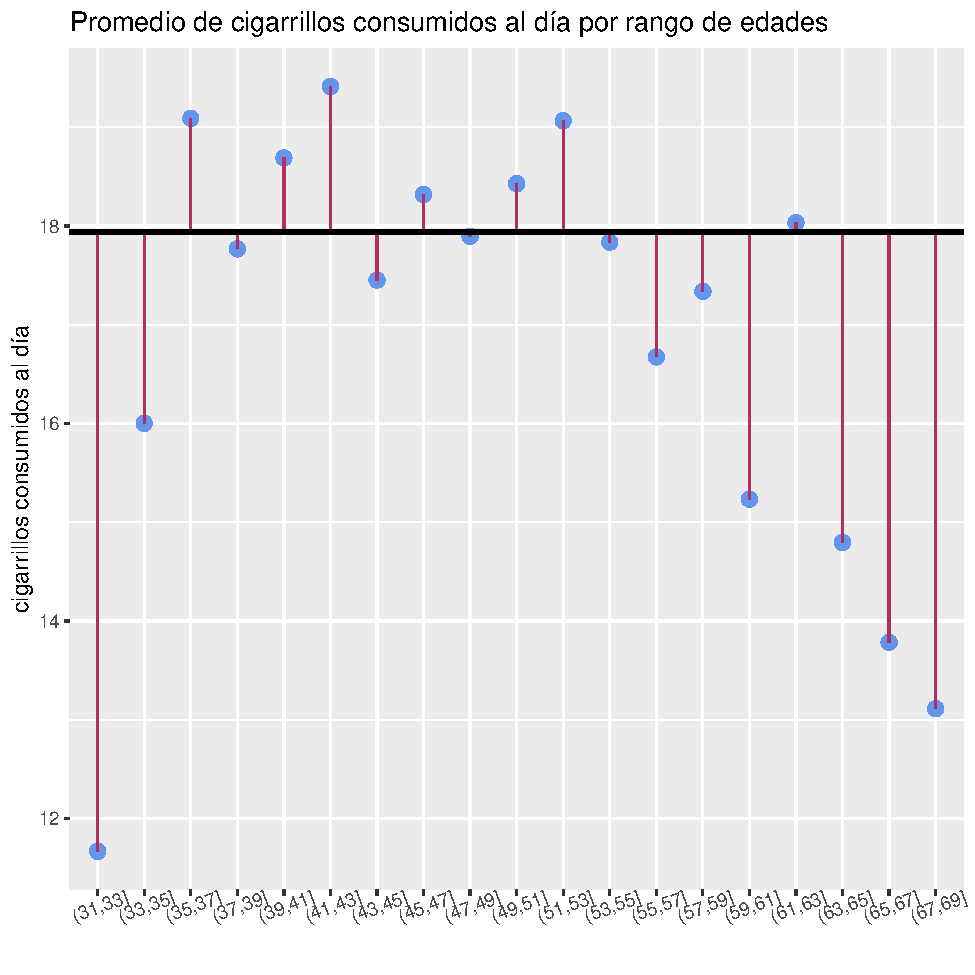
\includegraphics{Plantilla_Apa_files/figure-pdf/unnamed-chunk-1-1.pdf}

\subsection{Measures}\label{measures}

\subsection{Procedure}\label{procedure}

\section{Results}\label{results}

\section{Discussion}\label{discussion}

\subsection{Limitations and Future
Directions}\label{limitations-and-future-directions}

\subsection{Conclusion}\label{conclusion}

\section{References}\label{references}

\appendix

\section{Title for Appendix}\label{title-for-appendix}






\end{document}
